\documentclass{report}
\usepackage{cite}
\usepackage[utf8]{inputenc}
\usepackage[T1]{fontenc}
\usepackage{graphicx}
\usepackage{newtxtext}
\usepackage[a4paper, margin=0.5in]{geometry}
\usepackage{fancyhdr}
\usepackage{hyperref}
\usepackage{listings}
\usepackage{xcolor}
\usepackage{caption}


\definecolor{codegray}{rgb}{0.5,0.5,0.5}
\definecolor{codegreen}{rgb}{0,0.6,0}
\definecolor{codeblue}{rgb}{0,0,0.8}
\definecolor{codeback}{rgb}{0.95,0.95,0.92}

\lstdefinestyle{mystyle}{
    backgroundcolor=\color{codeback},
    commentstyle=\color{codegreen},
    keywordstyle=\color{codeblue},
    numberstyle=\tiny\color{codegray},
    stringstyle=\color{red},
    basicstyle=\ttfamily\footnotesize,
    breakatwhitespace=false,
    breaklines=true,
    captionpos=b,
    keepspaces=true,
    numbers=left,
    numbersep=5pt,
    showspaces=false,
    showstringspaces=false,
    showtabs=false,
    tabsize=2
}

\lstset{style=mystyle}


\setcounter{tocdepth}{4}
\setcounter{secnumdepth}{4}





\pagestyle{fancy} 
\fancyhf{}
\fancyfoot[C]{\thepage} 


\begin{document}

\begin{titlepage}
    \begin{center}
        {\small \textbf{In The Name Of God}}

        \vspace{1cm}

        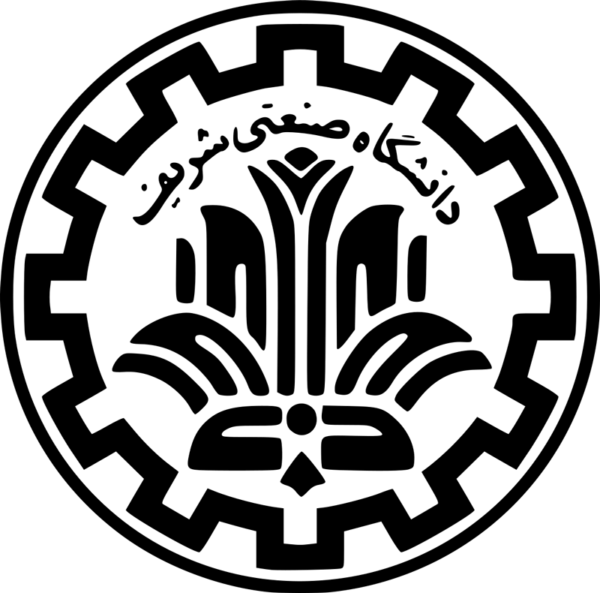
\includegraphics[width=0.3\textwidth]{logo.png} 

        \vspace{1cm}

        {\Huge Sharif University of Technology \\ Department of Electrical Engineering}

        \vspace{4cm}

        {\Large Data Network \\ 
        Instructor: Dr. Pakravan }
        
        \vspace{2cm}
        {\large \textbf{Linux Networking }}

        \vspace{4cm}

        {\Large Mohammad Javad Amin \\
        401211193}

        \vspace{3cm}

        {\Large Winter 2024}
    \end{center}
\end{titlepage}

\newpage

\tableofcontents

\newpage
\chapter*{Introduction}
\addcontentsline{toc}{chapter}{Introduction} 


\section*{Network Hypervisors}
\addcontentsline{toc}{section}{Network Hypervisors} 

A network hypervisor, also known as a network virtualization platform, is a software layer that abstracts and virtualizes network resources, similar to how a hypervisor virtualizes computing resources in server virtualization.
Network virtualization by decoupling the network control plane from the underlying hardware, allowing for more flexibility, scalability, and efficient resource utilization.\cite{1}
Here are some key reasons why network hypervisors are required:

\begin{enumerate}
  \item \textbf{Resource Abstraction:} Network hypervisors abstract physical network devices and resources, making it easier to manage and allocate network resources dynamically.
   This abstraction enables the creation of virtual networks that operate independently of the underlying physical infrastructure.

  \item \textbf{Isolation and Segmentation:} Network hypervisors facilitate the creation of isolated and segmented virtual networks on top of a shared physical network.
   This is crucial for multi-tenancy scenarios where different users or applications need to operate securely without interfering with each other.

  \item \textbf{Flexibility and Agility:} By decoupling the network control plane from hardware, network hypervisors provide greater flexibility and agility in managing network configurations.
  Changes can be made dynamically without requiring modifications to the underlying physical infrastructure.

  \item \textbf{Centralized Network Management:} Network hypervisors centralize the control and management of network resources, allowing administrators to define and enforce network policies from a central point.
  This centralized management simplifies network administration and reduces the likelihood of configuration errors.

  \item \textbf{Scalability:} Virtualized networks created by network hypervisors can easily scale up or down based on changing requirements.
  This scalability is essential in modern dynamic environments where workloads and network demands can vary rapidly.

  \item \textbf{Optimized Resource Utilization:} Network hypervisors contribute to optimized resource utilization by allowing multiple virtual networks to share the same physical infrastructure.
  This ensures that network resources are efficiently used, leading to cost savings and improved overall network performance.\cite{2}

\end{enumerate}
\begin{figure}[h] 
    \centering 
    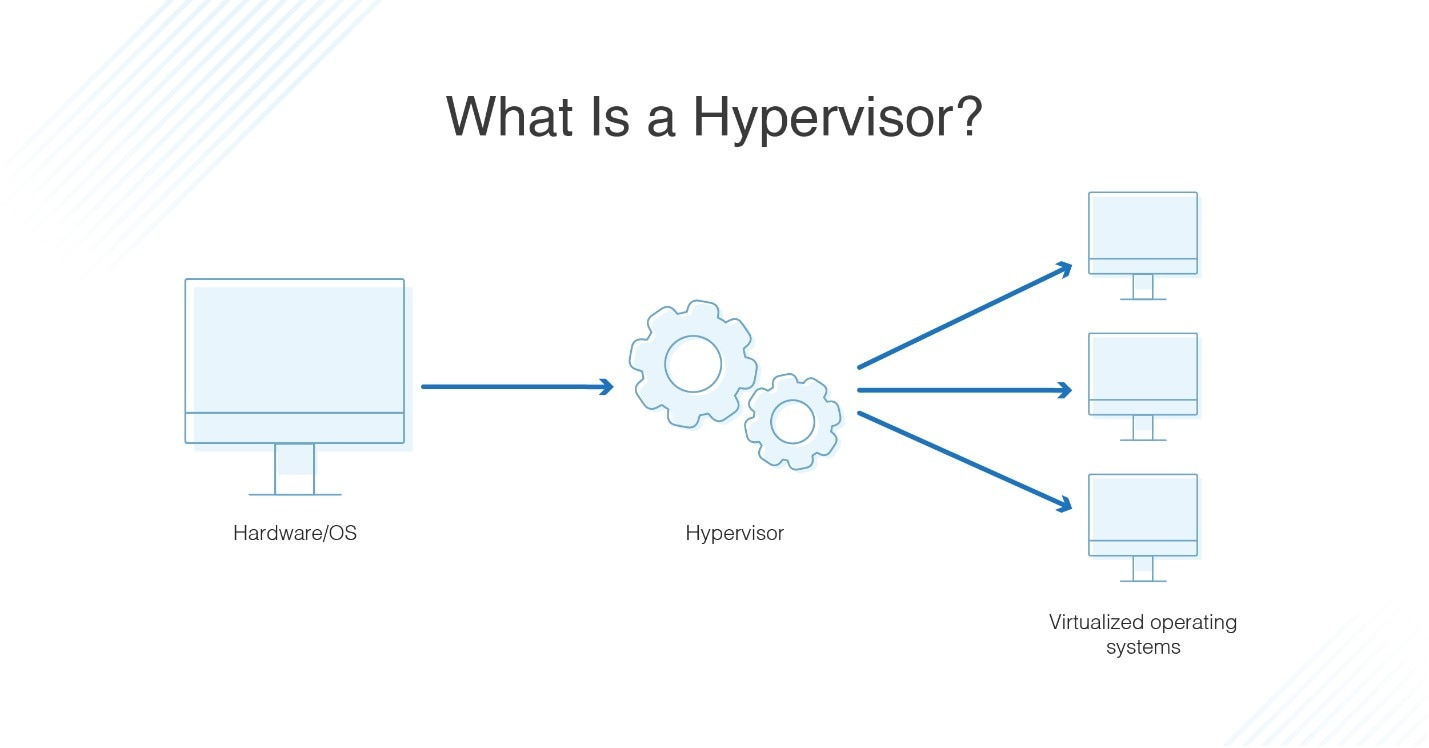
\includegraphics[width=0.6\textwidth]{1.jpg}
\end{figure} 


\section*{Virtualization in Networks}
\addcontentsline{toc}{section}{Virtualization in Networks} 

Virtualization in networks refers to the process of creating virtual instances or representations of physical network resources, such as servers, storage devices, or networks.
This technology enables the efficient utilization of resources, better scalability, and flexibility in managing network infrastructure.\cite{4}

\subsection*{Types of Virtualization in Networks:}

\begin{enumerate}
  \item \textbf{Server Virtualization:}
    Involves creating virtual instances of servers on a single physical server. Each virtual server operates independently with its own operating system.

  \item \textbf{Network Virtualization:}
    Focuses on creating virtual networks that operate independently of the physical network infrastructure. It allows for the segmentation of a physical network into multiple virtual networks.

  \item \textbf{Storage Virtualization:}
    Involves pooling and managing physical storage devices to create virtual storage resources. It provides flexibility in allocating storage space to different applications or users.

  \item \textbf{Desktop Virtualization:}
    Refers to the creation of virtual desktop environments that can be accessed remotely. Users can interact with a virtual desktop hosted on a server rather than a physical machine.

  \item \textbf{Application Virtualization:}
    Allows applications to run in isolated environments, separate from the underlying operating system. This enhances compatibility and reduces conflicts between applications.
\end{enumerate}

\begin{figure}[h] 
    \centering 
    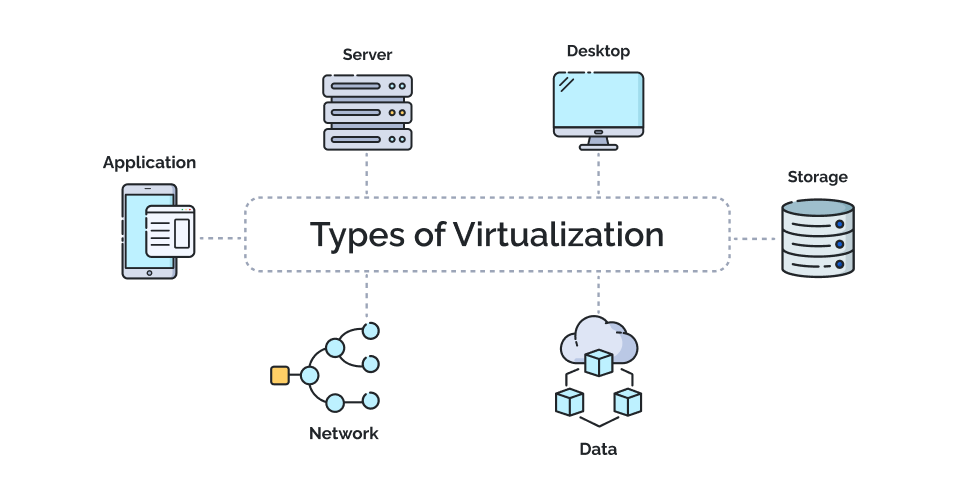
\includegraphics[width=0.6\textwidth]{3.png}
\end{figure} 

\subsection*{Role of Virtual Machines (VMs) in Virtualization:}

\begin{itemize}
  \item \textbf{Isolation and Independence:}
    Virtual Machines provide isolation between different operating systems and applications. Each VM operates independently, allowing for the simultaneous running of multiple operating systems on a single physical server.

  \item \textbf{Resource Optimization:}
    VMs enable efficient utilization of hardware resources by running multiple instances on the same physical server. This leads to improved resource utilization and cost savings.

  \item \textbf{Flexibility and Scalability:}
    VMs can be easily created, duplicated, or deleted, providing flexibility in managing workloads. This scalability allows for adapting to changing resource requirements without significant hardware changes.

  \item \textbf{Snapshot and Migration:}
    Virtualization platforms often offer features like snapshots, allowing for the capture of a VM's state at a specific point. This facilitates easy backup, recovery, and migration of VMs between physical servers.

  \item \textbf{Testing and Development:}
    VMs are widely used for testing and development purposes. Developers can create isolated environments to test applications without affecting the production environment.

  \item \textbf{Disaster Recovery:}
    Virtualization supports efficient disaster recovery strategies by enabling the quick restoration of VMs from backups. This helps minimize downtime and data loss in case of hardware failures or disasters.\cite{3}
\end{itemize}

\begin{figure}[h] 
    \centering 
    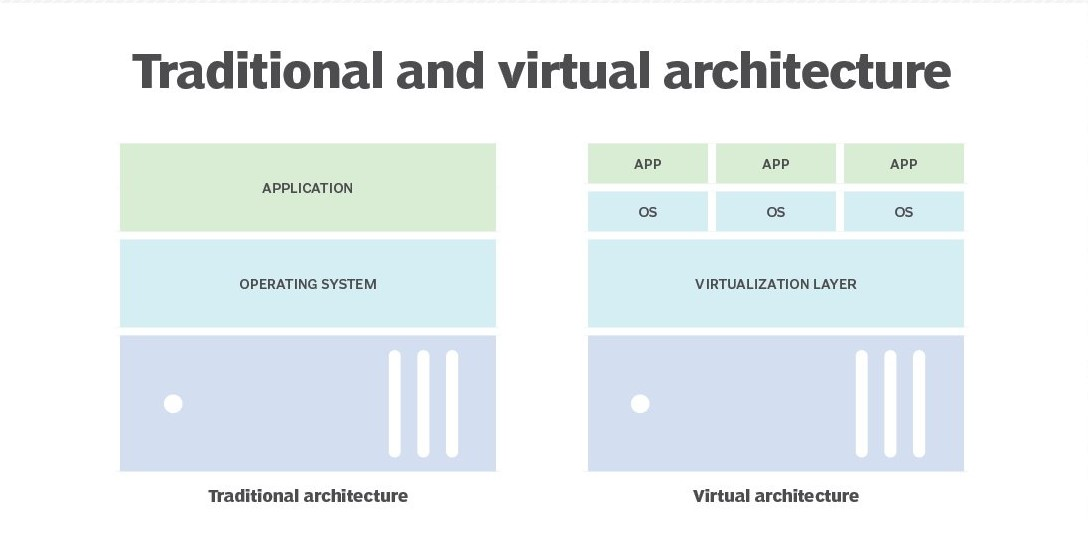
\includegraphics[width=0.5\textwidth]{2.jpg}
\end{figure} 


\chapter*{Basics of Linux Network Administration}
\addcontentsline{toc}{chapter}{Basics of Linux Network Administration} 

\section*{Network Interfaces}
\addcontentsline{toc}{section}{Network Interfaces} 






\begin{lstlisting}[language=bash]
$ ip link 
$ ip addr
\end{lstlisting}

\begin{figure}[h] 
  \centering 
  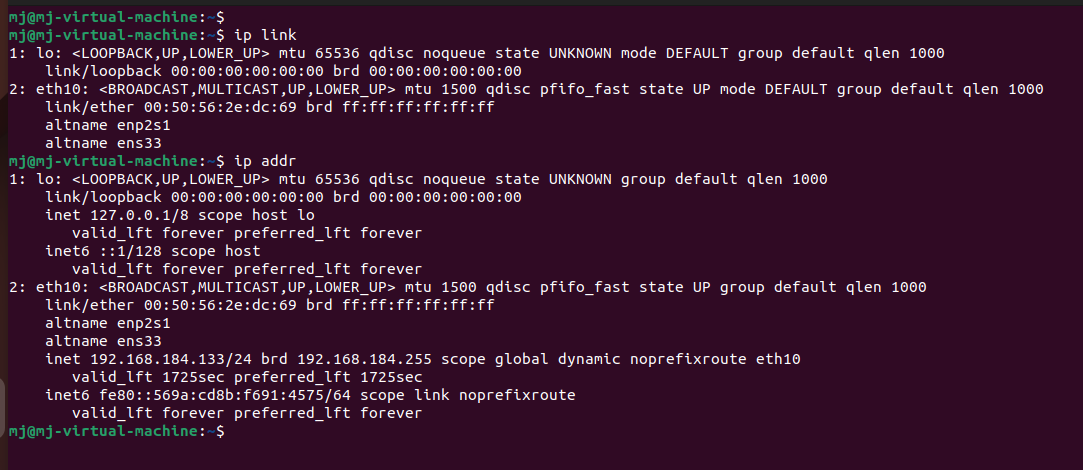
\includegraphics[width=0.9\textwidth]{11.png}
\end{figure} 



\begin{itemize}
  \item \textbf{lo (Loopback):}
    \begin{itemize}
      \item IP Address: 127.0.0.1
      \item MAC Address: Not explicitly shown, as the loopback interface does not have a physical MAC address associated with it.
    \end{itemize}
  
  \item \textbf{eth10 (Ethernet):}
    \begin{itemize}
      \item IP Address: 192.168.184.133
      \item MAC Address: 00:50:56:2e:dc:69
    \end{itemize}
\end{itemize}

The loopback interface (\texttt{lo}) is used for local communication within the host itself, and it always has the IP address 127.0.0.1.
The Ethernet interface (\texttt{eth10}) in a virtual machine is utilized for network communication,
facilitating connectivity with the host's physical network and enabling internet access.\cite{5} \\

\textbf{How the System Has Received Its IP Configuration:}
\begin{itemize}
  \item The loopback interface (\texttt{lo}) is assigned the loopback IP address (127.0.0.1) by default and does not require external configuration.
  \item The Ethernet interface (\texttt{eth10}) is assigned an IP address (192.168.184.133) through dynamic configuration (DHCP), as indicated by "dynamic" in the output. 
\end{itemize}


\section*{Probing the network between the local system and a destination}
\addcontentsline{toc}{section}{Probing the network between the local system and a destination} 

\subsection*{a. Traceroute}

\begin{lstlisting}[language=bash]
  $ traceroute www.google.com
\end{lstlisting}

This command will display the route that packets take to reach the google.com, showing the IP addresses of routers along the path.


\begin{figure}[h] 
  \centering 
  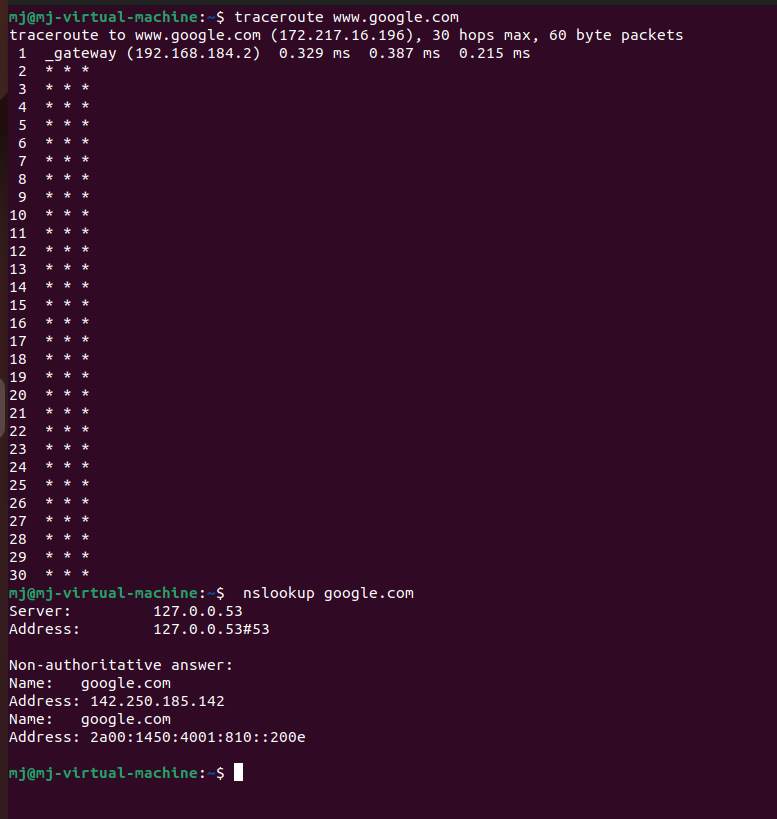
\includegraphics[width=0.9\textwidth]{12.png}
\end{figure} 



\subsubsection*{What Do Three Stars Represent?} 
We only see ***. This indicates that the router at that hop did not respond to the traceroute probe.

\begin{itemize}
  \item Some Routers Don’t Respond Because of the Overload:\\
  A router may be too busy to respond to the traceroute probe, treating it as a low-priority event. To check if this is the case, repeating the traceroute for the same destination multiple times may reveal whether the absence of *** was due to a temporary overload. If the path remains the same but *** disappears, it suggests a temporary overload. If the path changes, it may be because the overloaded router is temporarily avoided by other routers in the network.
  \item Some Routers Don’t Want to Respond:  \\
  Certain organizations configure their routers not to respond to traceroute requests to avoid revealing internal network details.\cite{6}

\end{itemize}


\subsection*{b. Routers Shown by Name:}
The routers shown by name instead of their IP addresses are resolved using reverse DNS lookup. When performing a traceroute, the tool attempts to resolve the IP addresses to corresponding hostnames. If the routers have reverse DNS entries, their names will be displayed.

\subsection*{c. Benefit of Knowing Routers in the Path:}
Being aware of the routers in the path provides several benefits:
\begin{itemize}
  \item \textbf{Network Troubleshooting:} It helps diagnose network issues by identifying the specific routers where packet loss or latency might be occurring.
  \item \textbf{Optimization:} Knowing the network path allows for optimization of routes, potentially improving network performance.
  \item \textbf{Security:} Understanding the route helps in identifying potential security risks or unauthorized network paths.
\end{itemize}

\subsection*{d. Find IP Address Record for 'google.com':}

\begin{lstlisting}[language=bash]
  $ nslookup google.com
\end{lstlisting}

or
\begin{lstlisting}[language=bash]
  $ dig +short google.com
\end{lstlisting}

This commands will provide the IP address associated with the 'google.com' server.


\section*{Network Interface Bonding}
\addcontentsline{toc}{section}{Network Interface Bonding}

\subsection*{a. Create a bond}

\begin{figure}[h] 
  \centering 
  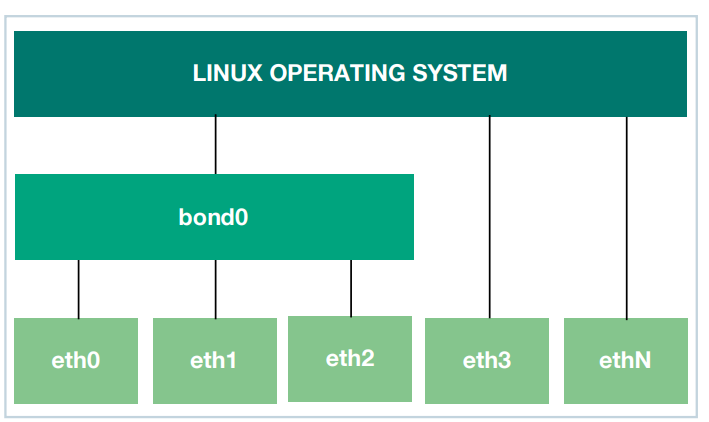
\includegraphics[width=0.9\textwidth]{21.png} 
  \captionsetup{labelformat=empty}
  \caption{Multiple Ethernet interfaces bonded into a single network interface.\cite{5}}
\end{figure} 

\begin{lstlisting}[language=bash]
# Create Interfaces
$ sudo ip link add eth0 type dummy
$ sudo ip link add eth1 type dummy
$ sudo ip link add eth2 type dummy

# All interface for adding to bond must be down

$ sudo modprobe bonding
$ sudo ip link add bond0 type bond mode 802.3ad

# Add eth0, eth1, and eth2 to the bond
$ sudo ip link set eth0 master bond0
$ sudo ip link set eth1 master bond0
$ sudo ip link set eth2 master bond0

# Activate the bond interface
$ sudo ip link set bond0 up

# To check the status of a bonded interface
$ cat /proc/net/bonding/bond0
\end{lstlisting}

This will create a bond interface named `bond0` consisting of the three physical interfaces (`eth0`, `eth1`, and `eth2`).

\begin{figure}[h] 
  \centering 
  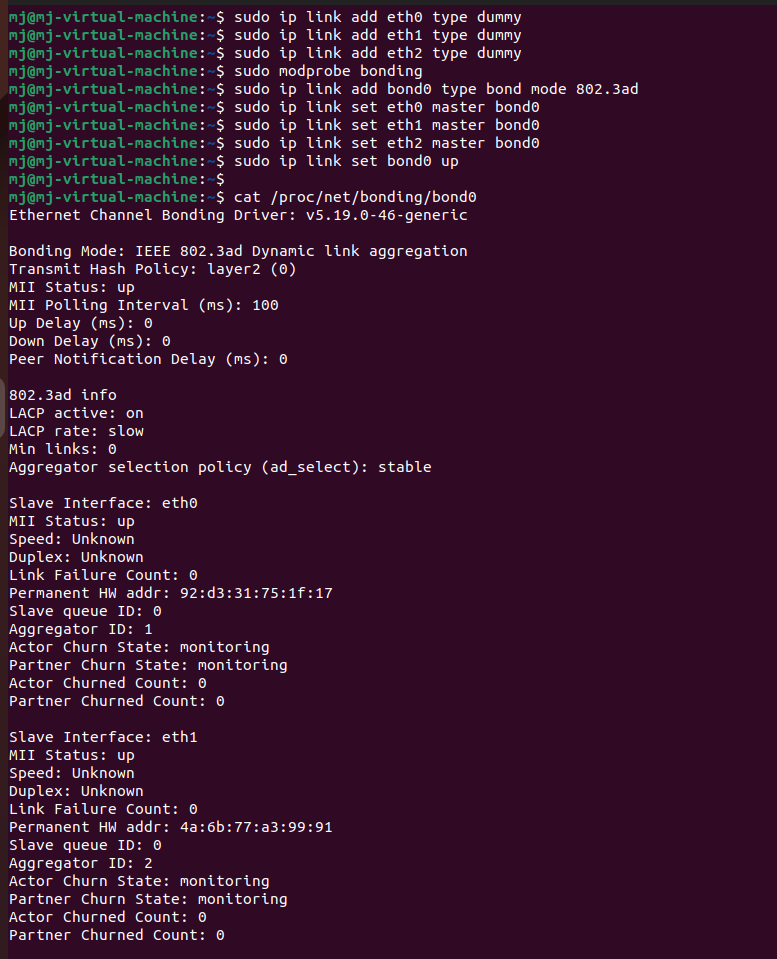
\includegraphics[width=0.7\textwidth]{13.png}
\end{figure} 

\subsection*{b. Linux Network Bonding Modes}
Bonding modes determine how network traffic is distributed across the member interfaces and how failover is handled.\\
Linux supports various bonding modes, each with specific characteristics:

\begin{itemize}
  \item \textbf{balance-rr:} The default mode is round-robin bonding, providing load balancing and fault tolerance.
  
  \item \textbf{active-backup:} Provides fault tolerance, allowing only one slave to be active at a time. If the active slave fails, another takes over.

  \item \textbf{balance-xor:} Provides fault tolerance and load balancing by transmitting based on hash.

  \item \textbf{broadcast:} Provides fault tolerance by transmitting everything on all slave interfaces.

  \item \textbf{802.3ad:} Follows the IEEE 802.3ad standard for dynamic link aggregation. It creates aggregation groups for links with the same speed and duplex to provide fault tolerance and load balancing. 802.3ad uses LACP to communicate with the other side of the bond.

  \item \textbf{balance-tlb:} Adaptive transmit load balancing that doesn't require any special switch support.

  \item \textbf{balance-alb:} Adaptive load balancing that doesn't require any special switch support due to its use of ARP negotiation.\cite{5}
\end{itemize}

The most common bonding modes are \textbf{active-backup} and \textbf{802.3ad}.


\chapter*{Understanding Linux Internetworking}
\addcontentsline{toc}{chapter}{Understanding Linux Internetworking} 

\section*{Layer 2 Internetworking on Linux Systems}
\addcontentsline{toc}{section}{Layer 2 Internetworking on Linux Systems} 

% \textbf{Bridging} \\

\subsection*{a. Create a bridge}


\begin{figure}[h] 
  \centering 
  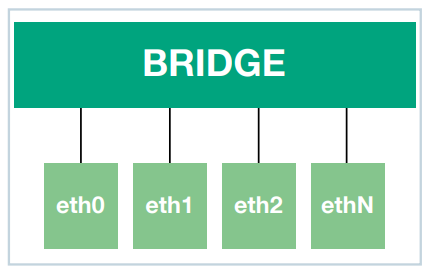
\includegraphics[width=0.5\textwidth]{22.png} 
  \captionsetup{labelformat=empty}
  \caption{Linux bridge configuration.\cite{5}}
\end{figure} 

\begin{lstlisting}[language=bash]
# Alreade create interfaces in last section
# Create the bridge 

# Create the bridge interface (br0)
$ sudo ip link add name br0 type bridge

# Add eth0, eth1, and eth2 to the bridge
$ sudo ip link set eth0 master br0
$ sudo ip link set eth1 master br0
$ sudo ip link set eth2 master br0

# Activate the bridge
$ sudo ip link set dev br0 up
\end{lstlisting}

This will create a bridge interface named `br0` and add the three physical interfaces (`eth0`, `eth1`, and `eth2`) to it.


\subsection*{b. MAC Address Table for the Bridge}
\begin{lstlisting}[language=bash]
  # Show MAC address table:
  $ sudo bridge fdb show
\end{lstlisting}

The following is the MAC address table for the network:

\begin{verbatim}
33:33:ff:91:45:75 dev eth10 self permanent
01:00:5e:00:00:01 dev eth10 self permanent
33:33:00:00:00:fb dev eth10 self permanent
01:00:5e:00:00:fb dev eth10 self permanent
33:33:00:00:00:01 dev eth10 self permanent
92:d3:31:75:1f:17 dev eth0 vlan 1 master br0 permanent
92:d3:31:75:1f:17 dev eth0 master br0 permanent
33:33:00:00:00:01 dev eth0 self permanent
4a:6b:77:a3:99:91 dev eth1 vlan 1 master br0 permanent
4a:6b:77:a3:99:91 dev eth1 master br0 permanent
33:33:00:00:00:01 dev eth1 self permanent
1e:7b:4b:09:ac:85 dev eth2 vlan 1 master br0 permanent
1e:7b:4b:09:ac:85 dev eth2 master br0 permanent
33:33:00:00:00:01 dev eth2 self permanent
33:33:00:00:00:01 dev br0 self permanent
01:00:5e:00:00:6a dev br0 self permanent
33:33:00:00:00:6a dev br0 self permanent
01:00:5e:00:00:01 dev br0 self permanent
a2:97:4c:80:5c:4a dev br0 vlan 1 master br0 permanent
a2:97:4c:80:5c:4a dev br0 master br0 permanent
\end{verbatim}

\subsubsection*{Analysis of the Table} 
The MAC address table provides information about which ports can reach specific MAC addresses in the bridge. Here are some key points from the table:

\begin{itemize}
  \item The table includes entries for different MAC addresses associated with various network interfaces (e.g., eth0, eth1, eth2, br0).
  \item Entries indicate the relationship between VLANs (virtual LANs) and the bridge (br0).
  \item The "permanent" status indicates that these entries are manually configured and will persist even after a reboot.
  \item The "self" designation implies that the MAC address is associated with the device itself.
\end{itemize}

\subsection*{c. Preventing Loops in Bridges}
To prevent loops in bridges, you can use the Spanning Tree Protocol (STP). STP is a protocol that prevents loops in network topologies by blocking redundant paths.
It's designed to identify and block any redundant paths to avoid loops.
\begin{lstlisting}[language=bash]
  # To enable STP on a bridge:
  $ sudo brctl stp br0 on
\end{lstlisting}


This command enables STP on the bridge `br0`. STP will then work to identify and block any redundant paths in the network.
\subsubsection*{Beneficial Fields in IP Packets for Loop Prevention}
The Time-To-Live (TTL) field in the IP header is crucial for loop prevention.
The TTL field is a counter that is decremented by each router that processes the packet.
If the TTL reaches zero, the packet is discarded. In the presence of a loop, the TTL would be decremented multiple times, and the packet would be dropped before causing network congestion or a broadcast storm.

\begin{figure}[h] 
  \centering 
  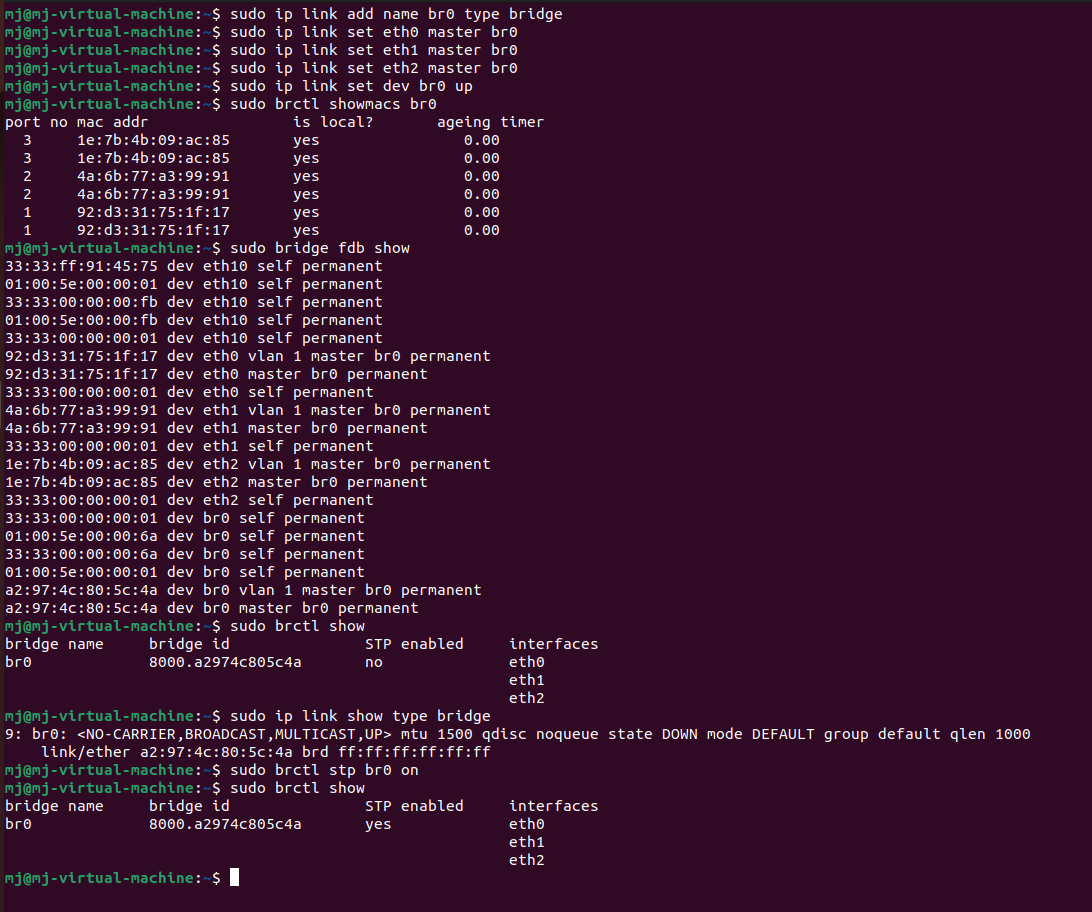
\includegraphics[width=0.7\textwidth]{16.png} 
\end{figure} 

\newpage
\section*{Layer 3 Internetworking View on Linux Systems}
\addcontentsline{toc}{section}{Layer 3 Internetworking View on Linux Systems} 

\subsection*{Neighbor Table}

\begin{lstlisting}[language=bash]
  # Show Neighbor table
  $ ip neigh show
\end{lstlisting}

The following is the neighbor table in the system:

\begin{figure}[h] 
  \centering 
  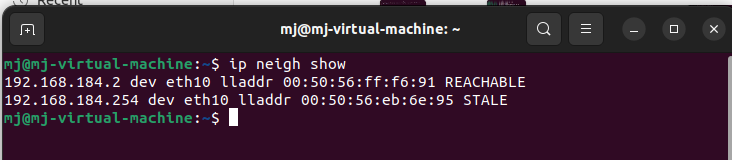
\includegraphics[width=0.9\textwidth]{17.png} 
\end{figure} 

\subsubsection*{Explanation of Fields in a Row}
Each row in the neighbor table provides information about a specific neighbor. Here's an explanation of the fields:

\begin{itemize}
  \item \textbf{192.168.184.2:} The IP address of the neighbor.
  
  \item \textbf{dev eth10:} The network interface through which the neighbor is reachable.

  \item \textbf{lladdr 00:50:56:ff:f6:91:} The Link Layer (MAC) address of the neighbor.

  \item \textbf{REACHABLE/STALE:} The state of the neighbor entry.\\
    - \textbf{REACHABLE:} The neighbor is currently reachable.\\
    - \textbf{STALE:} The neighbor entry is stale, meaning it might be outdated.

\end{itemize}

\subsection*{IP Routing}
\subsubsection*{a. Show the Routing Table}

\begin{lstlisting}[language=bash]
  # Show routing table
  $ ip route show
\end{lstlisting}

The following is the routing table in the system:

\begin{verbatim}
default via 192.168.184.2 dev eth10 proto dhcp src 192.168.184.133 metric 100 
192.168.184.0/24 dev eth10 proto kernel scope link src 192.168.184.133 metric 100
\end{verbatim}

\paragraph*{Explanation of Fields in a Row:\\} 
Each row in the routing table provides information about a specific route. 
Here's an explanation of the fields:

\begin{itemize}
  \item \textbf{default:} This route is the default route, used when no more specific route is found for a destination. It serves as the gateway of last resort.

  \item \textbf{via 192.168.184.2 dev eth10:} Traffic to destinations not covered by more specific routes will be sent via the gateway with IP address 192.168.184.2 through the network interface eth10.

  \item \textbf{proto dhcp:} The protocol used to obtain this route. In this case, it's obtained through DHCP.

  \item \textbf{src 192.168.184.133:} The source IP address associated with this route.

  \item \textbf{metric 100:} The metric or cost associated with the route. Lower values indicate higher priority.

  \item \textbf{192.168.184.0/24 dev eth10 proto kernel scope link src 192.168.184.133 metric 100:} This row represents a route to the local network (192.168.184.0/24) directly connected to the eth10 interface.

\end{itemize}

\subsubsection*{b. Role of the Default Route}
The \textbf{default route} serves as the gateway of last resort.
When a system needs to send a packet to a destination for which it doesn't have a more specific route, it uses the default route. 


\subsubsection*{c. Creating a Static Route and Making it Persistent}

\begin{lstlisting}[language=bash]
# Create a static route
$ sudo ip link set dev eth1 up
$ sudo ip route add 192.168.1.1 dev eth1
\end{lstlisting} 

This adds a static route saying that the network at 192.168.1.1 is reachable via the eth1 interface.

To make this route persistent after restarting the host, you can add the route information to a configuration file.
\begin{lstlisting}[language=bash]
  # Write a script
  $ sudo nano /etc/network/if-up.d/custom-routes
  $ sudo chmod +x /etc/network/if-up.d/custom-routes
\end{lstlisting}

This script will be executed whenever a network interface is brought up.

\begin{figure}[h] 
  \centering 
  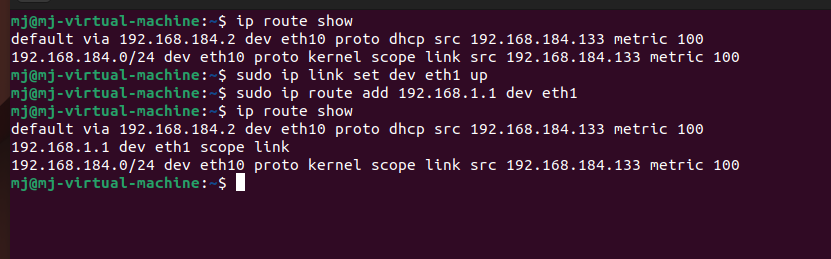
\includegraphics[width=0.9\textwidth]{18.png} 
\end{figure} 



\section*{Virtual LANs (VLANs)}
\addcontentsline{toc}{section}{Virtual LANs (VLANs)} 

\begin{figure}[h] 
  \centering 
  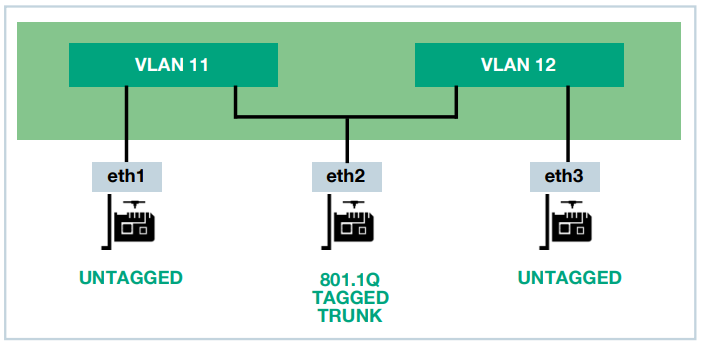
\includegraphics[width=0.9\textwidth]{23.png} 
  \captionsetup{labelformat=empty}
  \caption{Tagged and untagged VLAN traffic.\cite{5}}
\end{figure} 
  

\subsubsection*{a. Creating VLANs with Bridges}

\begin{lstlisting}[language=bash]
# Load the 8021q module
sudo modprobe 8021q

# Create a bridge named br0 with VLAN filtering enabled
sudo ip link add br0 type bridge vlan_filtering 1

# Attach eth1, eth2, and eth3 to the br0 bridge
sudo ip link set eth1 master br0
sudo ip link set eth2 master br0
sudo ip link set eth3 master br0

# Add VLAN 11 to eth1 with untagged traffic 
sudo bridge vlan add dev eth1 vid 11 pvid untagged

# Add VLAN 12 to eth3 with untagged traffic 
sudo bridge vlan add dev eth3 vid 12 pvid untagged

# Add VLAN 11 to eth2
sudo bridge vlan add dev eth2 vid 11

# Add VLAN 12 to eth2
sudo bridge vlan add dev eth2 vid 12

# Bring up the bridge and associated interfaces
sudo ip link set up dev br0
sudo ip link set up dev eth0
sudo ip link set up dev eth1
sudo ip link set up dev eth2
sudo ip link set up dev eth3
\end{lstlisting} 

This setup places eth1 in VLAN11, eth3 in VLAN12, and eth2 in both VLANs\cite{5}

\begin{figure}[h] 
  \centering 
  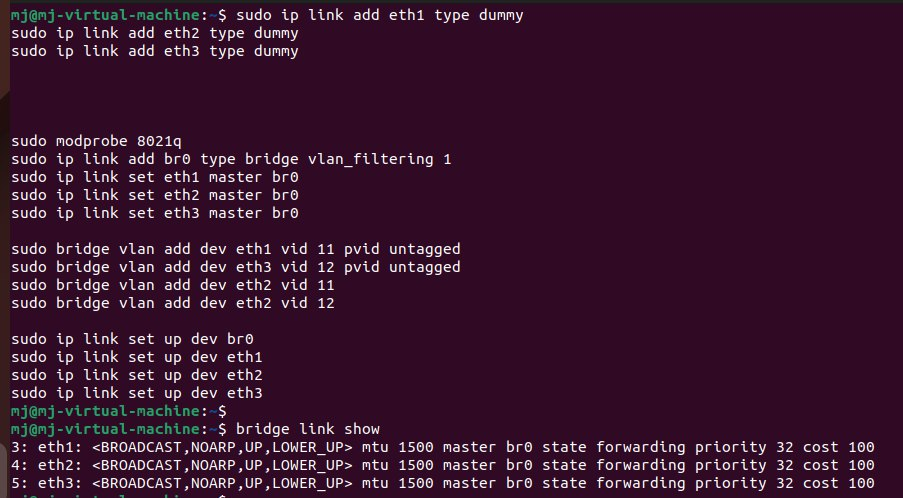
\includegraphics[width=0.9\textwidth]{19.jpg} 
\end{figure} 


\subsubsection*{b. Trunks}

In networking, a trunk is a communication path between two network devices where multiple VLANs can travel.
Trunks are often used to carry traffic for multiple VLANs over a single physical link.

In the given scenario, eth2 is configured as a tagged trunk because it carries traffic for both VLAN11 and VLAN12.
The VLAN tagging allows the switch or other network devices to distinguish between the VLANs.

\subsubsection*{c. MAC Address Tables in 3 VLANs}
The MAC address tables for VLANs 11, 12, and the default/native VLAN are different. 
Each VLAN operates as a separate broadcast domain, and the MAC address table is specific to each VLAN.
Devices in one VLAN are not aware of devices in other VLANs, and the switches maintain separate MAC address tables for each VLAN.
So, the MAC address tables for VLAN11, VLAN12, and the default VLAN are contain the MAC addresses of devices within their respective VLANs, but not devices in other VLANs.
\newpage
\subsubsection*{d. Screenshots}
\begin{figure}[h] 
  \centering 
  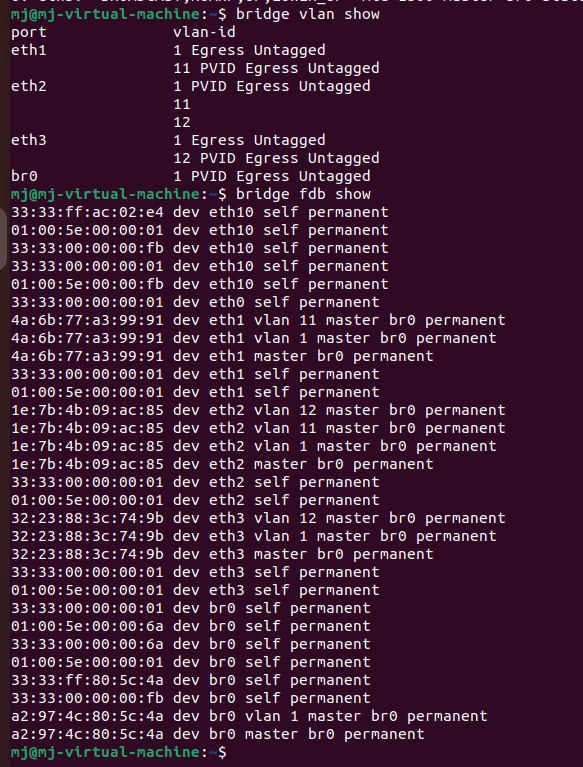
\includegraphics[width=0.8\textwidth]{31.jpg} 
\end{figure} 



\chapter*{Namespaces in linux}
\addcontentsline{toc}{chapter}{Namespaces in linux} 

\section*{a. Linux Namespaces}

In Linux, namespaces are a feature that allows different processes to have isolated views of various system resources.
They provide a way to partition system resources among different processes, creating a form of process-level virtualization.
Here are some of the main namespaces in Linux and a brief explanation of each:

\begin{itemize}

  \item \textbf{PID Namespace (pid):}
    \begin{itemize}
      \item \textbf{Application:} Provides isolation for process IDs (PIDs).
      \item \textbf{Explanation:} Processes in different PID namespaces have their own set of PIDs, meaning they may see different processes as having PID 1, for example. This can be useful for process isolation and management.
    \end{itemize}

  \item \textbf{Network Namespace (net):}
    \begin{itemize}
      \item \textbf{Application:} Isolates network-related resources.
      \item \textbf{Explanation:} Processes in different network namespaces have their own network stack, interfaces, routing tables, and firewall rules. This is useful for creating network-isolated environments, similar to virtual machines.
    \end{itemize}

  \item \textbf{Mount Namespace (mnt):}
    \begin{itemize}
      \item \textbf{Application:} Isolates the filesystem mount points.
      \item \textbf{Explanation:} Processes in different mount namespaces have their own view of the filesystem. Changes to mounts in one namespace do not affect others. This is commonly used in containerization to provide a private filesystem space for each container.
    \end{itemize}

  \item \textbf{IPC Namespace (ipc):}
    \begin{itemize}
      \item \textbf{Application:} Provides isolation for Inter-Process Communication (IPC) resources.
      \item \textbf{Explanation:} Processes in different IPC namespaces have their own System V IPC objects (like message queues, semaphores, and shared memory segments). This allows isolation and independence between processes using these communication mechanisms.
    \end{itemize}

  \item \textbf{UTS Namespace (uts):}
    \begin{itemize}
      \item \textbf{Application:} Isolates the hostname and NIS domain name.
      \item \textbf{Explanation:} Processes in different UTS namespaces have their own hostname and NIS domain name. This is useful for providing a distinct identity to processes running in separate namespaces.
    \end{itemize}

  \item \textbf{User Namespace (user):}
    \begin{itemize}
      \item \textbf{Application:} Provides isolation for user and group IDs.
      \item \textbf{Explanation:} Processes in different user namespaces have their own view of user and group IDs. This is crucial for user namespace mapping, especially in the context of containerization, where it allows processes to have different UID/GID mappings inside and outside a container.
    \end{itemize}

  \item \textbf{Cgroup Namespace (cgroup):}
    \begin{itemize}
      \item \textbf{Application:} Provides isolation for control group (cgroup) hierarchies.
      \item \textbf{Explanation:} Processes in different cgroup namespaces have their own view of the cgroup hierarchy. This is used to isolate resource management policies among different groups of processes.
    \end{itemize}

\end{itemize}

These namespaces collectively contribute to the lightweight process isolation and containerization features in Linux. 
Tools like Docker and Kubernetes extensively leverage these namespaces to create isolated and portable environments for applications.
Each namespace provides a way to separate and control specific aspects of a process's view of the system.\cite{8}

\subsubsection*{Comparison between VLANs and Network Namespaces(additional information)}

\begin{itemize}
  \item \textbf{Layer of Operation:} VLANs operate at Layer 2, dealing with MAC addresses and broadcast domains, while network namespaces operate at Layer 3 and above, dealing with IP addresses and complete network stacks.
  
  \item \textbf{Scope of Isolation:} VLANs primarily isolate broadcast domains, allowing devices within the same VLAN to communicate. Network namespaces provide a more comprehensive isolation, separating entire network stacks.
  
  \item \textbf{Configuration:} VLANs are configured on network switches. In contrast, network namespaces are configured and managed by the operating system kernel.
  
  \item \textbf{Use Case:} VLANs are commonly used in large-scale enterprise networks to segment traffic and improve network efficiency. Network namespaces find application in containerization and virtualization for process isolation, creating independent network environments for applications or services.\cite{9}
\end{itemize}

\subsection*{b. Create Two Network Namespaces}

\begin{figure}[h] 
  \centering 
  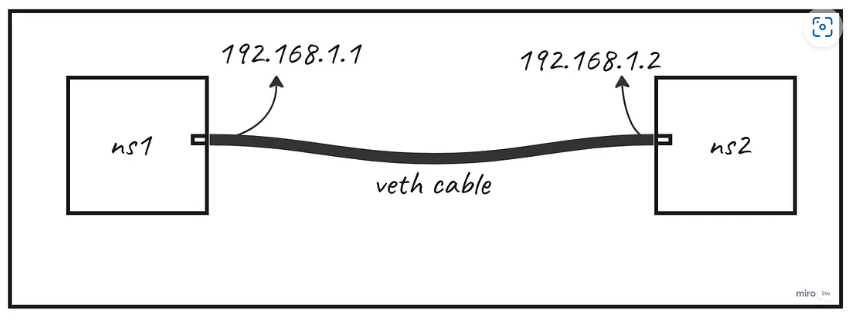
\includegraphics[width=0.9\textwidth]{24.png} 
  \captionsetup{labelformat=empty}
  \caption{Two namespaces connected witha a veth cable.\cite{9}}
\end{figure} 


\begin{lstlisting}[language=bash]
# Create network namespaces
$ sudo ip netns add ns1
$ sudo ip netns add ns2
\end{lstlisting}

\subsection*{c. Create and Configure Veth Cable}

\begin{lstlisting}[language=bash]
# Create a virtual Ethernet pair
$ sudo ip link add eth1 type veth peer name eth2
\end{lstlisting}

\subsection*{d. Connect Veth Cable with Each Namespace}

\begin{lstlisting}[language=bash]
# Move each end of the pair to its respective namespace
$ sudo ip link set eth1 netns ns1
$ sudo ip link set eth2 netns ns2
\end{lstlisting}

\subsection*{e. Bind IP Address with Interfaces}

\begin{lstlisting}[language=bash]
# Assign IP addresses to the interfaces
$ sudo ip netns exec ns1 ip addr add 192.168.1.1/24 dev eth1
$ sudo ip netns exec ns2 ip addr add 192.168.1.2/24 dev eth2
\end{lstlisting}

Now, attempt to ping one node from another:

\begin{lstlisting}[language=bash]
# Ping
$ sudo ip netns exec ns1 ping 192.168.1.2
\end{lstlisting}

\textbf{Observation:} The nodes are not reachable because we haven't activated the interfaces yet.

\subsection*{f. Activate Interfaces}

\begin{lstlisting}[language=bash]
# Bring up the interfaces
$ sudo ip netns exec ns1 ip link set eth1 up
$ sudo ip netns exec ns2 ip link set eth2 up
\end{lstlisting}

Now, attempt to ping again:

\begin{lstlisting}[language=bash]
# Ping
$ sudo ip netns exec ns1 ping 192.168.1.2
\end{lstlisting}

\textbf{Observation:} The nodes are reachable now.

\subsection*{g. Write Bash Script}

Create a bash script named \texttt{my-script.sh} use nano:
\begin{lstlisting}[language=bash]
  $ nano my_script.sh
\end{lstlisting}

\begin{lstlisting}[language=bash]
  #!/bin/bash

  if [ "$#" -ne 2 ]; then
      echo "Usage: $0 <node1> <node2>"
      exit 1
  fi
  
  node1=$1
  node2=$2
  
  # Create network namespaces
  sudo ip netns add $node1
  sudo ip netns add $node2
  
  # Create a virtual Ethernet pair
  sudo ip link add eth1 type veth peer name eth2
  
  # Move each end of the pair to its respective namespace
  sudo ip link set eth1 netns $node1
  sudo ip link set eth2 netns $node2
  
  # Assign IP addresses to the interfaces
  sudo ip netns exec $node1 ip addr add 192.168.1.1/24 dev eth1
  sudo ip netns exec $node2 ip addr add 192.168.1.2/24 dev eth2
  
  # Bring up the interfaces
  sudo ip netns exec $node1 ip link set eth1 up
  sudo ip netns exec $node2 ip link set eth2 up
  
  # Ping from node1 to node2
  sudo ip netns exec $node1 ping 192.168.1.2
\end{lstlisting}

Make it executable:

\begin{lstlisting}[language=bash]
chmod +x my_script.sh
\end{lstlisting}

Run the script:

\begin{lstlisting}[language=bash]
./my_script.sh node1 node2
\end{lstlisting}

\subsection*{h. Ping 8.8.8.8 from Each Namespace}

\begin{lstlisting}[language=bash]
sudo ip netns exec ns1 ping 8.8.8.8
sudo ip netns exec ns2 ping 8.8.8.8
\end{lstlisting}

\textbf{Observation:} 8.8.8.8 may not be reachable. The issue is due to the lack of internet access in the isolated namespaces.

\subsubsection*{Solution for Internet Access in Namespaces}

To enable internet access, you need to set up network address translation (NAT) and forwarding in the main network namespace.\cite{9}


\chapter*{Acknowledgments}
\addcontentsline{toc}{chapter}{Acknowledgments} 

I extend my sincere appreciation to ChatGPT for its invaluable assistance in the writing process of this report.
The ability to generate LaTeX-formatted content and provide insightful answers to questions has significantly contributed to the completion of this work.
I express my gratitude for the support provided throughout this endeavor.


\renewcommand{\bibname}{References}
\cleardoublepage  
\phantomsection   
\addcontentsline{toc}{chapter}{\bibname}
\bibliographystyle{IEEEtran}
\bibliography{ref.bib}


\end{document}